% vim: set tw=80 aw sw=2 sts=2 noet:
\documentclass{beamer}

%\includeonlyframes{c} % speeding up compilation speed during debug

\usepackage[utf8x]{inputenc} % diacritice
\usepackage[english]{babel}
\usepackage{hyperref}        % \url{http://...} | \href{http://...}{Nume Link}

\mode<presentation>
\usetheme{SCS}

% Pentru a afisa (cont.) la slide-uri prea lungi split-uite pe mai multe pag
\setbeamertemplate{frametitle continuation}[from second]
% Pentru a modifica modul de afisare al numerelor de slide
\setbeamertemplate{footline}[frame number]

\title{The Silent Leak}
\subtitle{Defeating iOS Default Caching (OWASP M9)}
% Folositi institutul pentru conducatorul stiintific
\institute{Security of Mobile Devices Lab, UPB}
\author{Horia-Alexandru Banica}

\begin{document}

{
  % Schimbam fundalul aici pentru a avea slide-ul cu logo-urile
  \usebackgroundtemplate{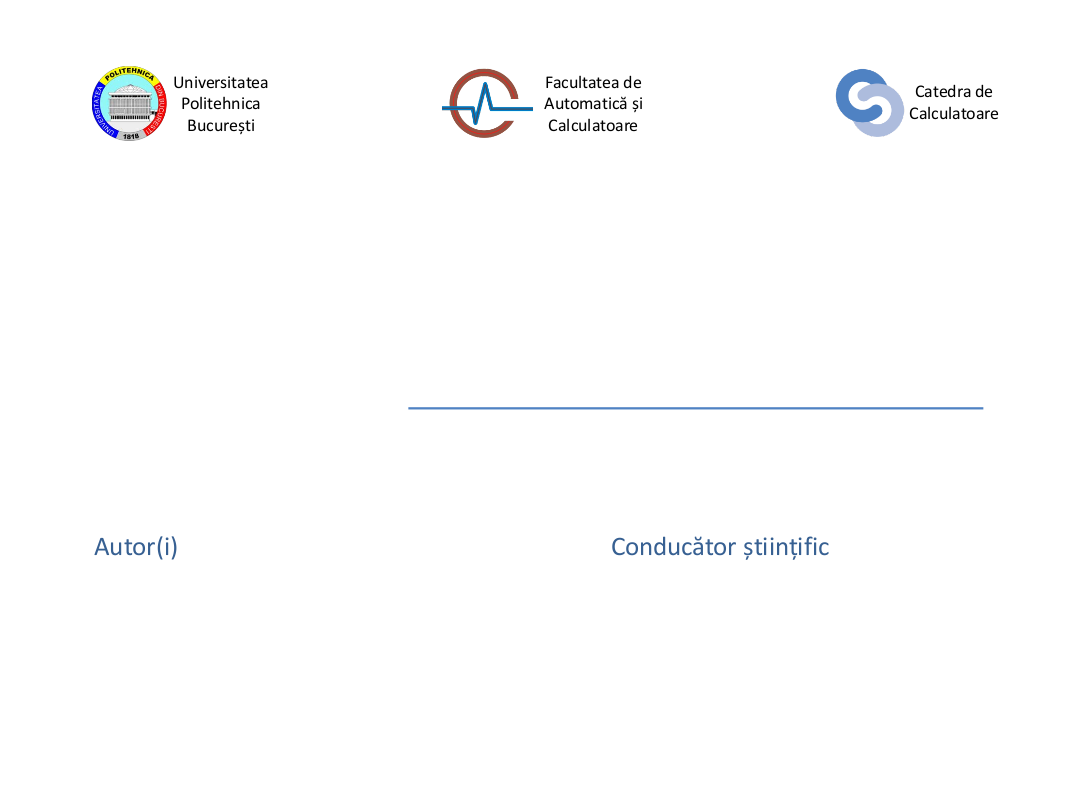
\includegraphics[width=\paperwidth]{title}}
  \frame{\titlepage}
}

\begin{frame}{Agenda}
  \begin{itemize}
    \item \textbf{Introduction:} The Illusion of Data at Rest
    \item \textbf{The Vulnerability:} \texttt{URLSession} Default Behavior
    \item \textbf{The Impact:} From Pokédex to Enterprise Data
    \item \textbf{The Solution:} Preventing Leaks in Code
    \item \textbf{Technical Demo}
  \end{itemize}
\end{frame}

\begin{frame}{Introduction: The Security Illusion (OWASP M9)}
  \begin{itemize}
    \item \textbf{HTTPS} secures data \textit{in transit} (preventing Man-in-the-Middle attacks).
    \item However, developers often neglect the state of data \textit{at rest}.
    \item \textbf{OWASP Mobile Top 10 - M9 (Insecure Data Storage)} covers the accidental storage of sensitive data directly on the device.
    \item Native Apple frameworks prioritize performance (load speed) over strict data security by default.
  \end{itemize}
\end{frame}

\begin{frame}{The Vulnerability: Silent Caching in iOS}
  \begin{itemize}
    \item The \texttt{URLSession.shared} object \textbf{automatically} saves decrypted HTTP responses directly to the physical disk.
    \item Disk Location: \texttt{Library/Caches/<bundle-id>/}
    \item Modern iOS 26+ caching architecture:
    \begin{itemize}
        \item \textbf{\texttt{Cache.db} (SQLite):} Stores only the request metadata and assigns a UUID.
        \item \textbf{\texttt{fsCachedData/}:} A hidden folder where the raw payload file is dumped (unencrypted JSON, images).
    \end{itemize}
  \end{itemize}
\end{frame}

\begin{frame}{Impact and Solution}
  \begin{itemize}
    \item \textbf{Enterprise Impact:} If cache is mismanaged, an app will leak OAuth Tokens, private messages, medical records, and financial data to the disk.
    \item \textbf{Solution 1 (Global):} Disable cache memory for the entire app:
    \par\smallskip
    \texttt{URLCache.shared.diskCapacity = 0}
    \item \textbf{Solution 2 (Recommended):} Use ephemeral sessions. This forces the OS to keep data \textit{strictly in RAM}:
    \par\smallskip
    \texttt{let config = URLSessionConfiguration.ephemeral}
    \par
    \texttt{let session = URLSession(configuration: config)}
  \end{itemize}
\end{frame}

\begin{frame}{Technical Demo}
  \begin{center}
    \Large \textbf{Live: Extracting Data from the Simulator}\par
    \vspace{2em}
    \normalsize App Target: \texttt{test.demo-vuln-lab4}\par
    \vspace{1em}
    Step 1: Generate network traffic\par
    Step 2: Force disk write (Backgrounding the app)\par
    Step 3: Bypass \texttt{Cache.db} and expose JSON from \texttt{fsCachedData}
  \end{center}
\end{frame}

\end{document}
